\section{Informal presentation of the {calculus}}\label{sect:informal}
Syntax and types are given in \refToFigure{syntax}.  We assume sets of \emph{variables} $\x$, $\y$, $\z$, \emph{class names} $\C$, \emph{field names} $\f$, and \emph{method names} $\m$. 
We adopt the convention that a metavariable which ends by $\metavariable{s}$ is implicitly defined as a (possibly empty) sequence, {for example} {$\decs$ is defined by $\produzioneinline{\decs}{\epsilon\mid \dec\ \decs}$}, where $\epsilon$ denotes the empty sequence.

\begin{figure}
\framebox{{\small \begin{grammatica}
\produzione{\cd}{\terminale{class}\ \C\ \terminale{\{}\fds\ \mds \terminale{\}}}{class declaration}\\*
\produzione{\fd}{
\Field{\Type{\imm}{\C}}{\f}
\mid
\Field{\Type{\mutable}{\C}}{\f}\mid\Field{\intType}{\f}}{field declaration}\\*
\produzione{\md}{\MethDec{\T}{\m}{{\mu}}{\T_1\,\x_1,\ldots,\T_n\,\x_n}{\e}}{method declaration}\\*
\produzione{\e}{\x\mid\FieldAccess{\e}{\f}\mid\MethCall{\e}{\m}{\es}\mid\FieldAssign{\e}{\f}{\e}\mid\ConstrCall{\C}{\es}\mid\Block{\decs}{\e}}{expression}\\*
\produzione{\dec}{\Dec{\T}{\x}{\e}}{variable declaration}\\*
\\
\produzione{\T}{\Type{\mu}{\C}\mid\intType}{type}\\*
\produzione{\mu}{\mutable\mid\imm\mid\capsule\mid\lent\mid\readable}{{(type)} qualifier}\\*
\\
\produzione{\dv}{\Dec{\T}{\x}{\stVal}}{evaluated declaration}\\
%\produzione{{\valPrime,}\val}{{\x\mid\ConstrCall{\C}{\vals}\mid\Block{\dvs}{\val}}}{value}\\*
\produzione{\stVal}{\ConstrCall{\C}{\xs}\mid\Block{\dvs}{\x}\mid\Block{\dvs}{\ConstrCall{\C}{\xs}}}{\storableVal}
\end{grammatica}
}}
\caption{Syntax and types}\label{fig:syntax}
\end{figure}

The syntax mostly follows Java and Featherweight Java (FJ) \cite{IgarashiEtAl01}. A class declaration consists of a class name, a sequence of field declarations and a sequence of method declarations. A field declaration consists of a field type and a field name.
 A method declaration consists, as in FJ, of a return type, a method name, a list of parameter names with their types, and a body which is an expression. {However, there is an additional component: the type qualifier for $\this$, which is {written as additional (first) element of the parameter list}.}
  As in FJ, we assume for each class a canonical constructor whose parameter list exactly corresponds to the class fields, and we assume no multiple declarations of classes in a class table, fields and methods in a class declaration. 

For expressions, in addition to the standard constructs of imperative object-oriented languages, we have 
\emph{blocks}, which are sequences of variable declarations, followed by a \emph{body} which is an expression.
Variable declarations consist of a type, a variable and an initialization expression. 
Types are class names decorated by a \emph{{(type)} qualifier}. We also include $\intType$ as an example of primitive type, but we do not formally model related operators used in the examples, such as integer constants and sum. We assume no multiple declarations for variables in a block, that is, $\decs$ can be seen as a map from variables into declarations, and we use the notations $\dom{\decs}$ and $\decs(\x)$.

Blocks are a fundamental construct of our {calculus}, since sequences of local variable declarations, when evaluated, are used to directly represent store  in the language itself. A declaration is evaluated if its initialization expression is a \emph{right-value}, that is, either an \emph{object state} (a constructor invocation where arguments are references) or a block in which declarations are evaluated and the body is a reference or an object state.

For instance\footnote{In the examples, we omit for readability the brackets of the outermost block.}, assuming that class \lstinline{B} has a $\mutable$ field of type \lstinline{B}{, in the block}:
\begin{lstlisting}
mut B x= new B(y); mut B y= new B(x); x 
\end{lstlisting}
the two declarations can be seen as a store where \lstinline{x} denotes an object of class \lstinline{B} whose field is \lstinline{y}, and conversely, as shown in \refToFigure{es1}(a).
\begin{figure}[ht]
\begin{center}
\includegraphics
[width=1\textwidth]
{Es1e2.pdf}
\end{center}
\caption{Graphical representation of the store} \label{fig:es1}
\end{figure}
The whole block denotes a store with an entry point (graphically represented by a thick arrow). {In our graphical representation circles denote mutable references {(\lstinline{x}{} and \lstinline{y}{} in \refToFigure{es1})}, diamonds denote immutable references (\lstinline{z}{} and \lstinline{w}{} in \refToFigure{es1}(b)) and squares denote {capsule references}  (\lstinline{z}{} in \refToFigure{esRed2})}.
 
Stores are \emph{hierarchical}, rather than flat as it usually happens in models of imperative languages. 
For instance, assuming that class \lstinline{C}{} has two $\mutable$ \lstinline{D}{} and one $\imm$ \lstinline{D}{} fields,  and class \lstinline{D}{} has an integer field, the following is a store:
\begin{small}
\begin{lstlisting}
imm D z= new D(0);
imm C w= {mut D x= new D(1); mut D y= new D(2); new C(x,y,z)}  
\end{lstlisting}
\end{small}

Here, the {right-value} associated to \lstinline{w}{} is a block introducing local declarations, that is, in turn a store {with an entry point}, as shown in \refToFigure{es1}(b). 
The advantage of this hierarchical shape is that it models in a simple and natural way constraints about aliasing among objects, notably:
\begin{itemize}
\item the fact that an object is not referenced from outside some enclosing object is directly modeled by the block construct: for instance, the objects denoted by \lstinline{x}{} and \lstinline{y}{} can only be reached through \lstinline{w}{}
\item conversely, the fact that an object does not refer to the outside is modeled by the fact that the corresponding block is closed, that is, has no free variables\footnote{In other words, our calculus smoothly integrates memory representation with shadowing and $\alpha$-conversion.}: for instance, the object denoted by \lstinline{w}{} is not closed, since it refers to the external object \lstinline{z}{}.
\end{itemize}
%In the graphical representation, {variables in a grey circle are immutable references, others are mutable.}
In the graphical representation the reference corresponding to \lstinline{new C(x,y,z)}{} is anonymous.
Note also that, in this example, mutable variables in the local store of \lstinline{w}{} are not visible from the outside. This models in a natural way the fact that the portion of store denoted by \lstinline{w}{} is indeed immutable, as will be detailed in the sequel.

We illustrate now the meaning of the qualifiers $\mutable$, $\imm$, and $\capsule$.
A mutable variable refers to a portion of store that can be modified during execution. For instance, the block 
\begin{lstlisting}
mut B x= new B(y); mut B y= new B(x); x.f=x
\end{lstlisting}
reduces to
\begin{lstlisting}
mut B x= new B(x); mut B y= new B(x); x
\end{lstlisting}
We give a graphical representation of this reduction in \refToFigure{esRed1}
\begin{figure}[ht]
\begin{center}
\includegraphics[width=1\textwidth]{EsEsecuzione1.pdf}
\end{center}
\caption{Example of reduction (1)} \label{fig:esRed1}
\end{figure}
 where we
highlight in grey expressions which {are not reduced yet}. So in  (a) the body of the block is the expression \lstinline{x.f=x}{}, whose evaluation
modifies the field \lstinline{f}{} of \lstinline{x}{}, and returns \lstinline{x}{}. The result of the reduction is shown in (b). 

Variables declared immutable, instead, {refer to a portion of store which cannot be modified.}
 Immutability is \emph{deep/full}, that is, all the nodes in the reachable object graph of an immutable reference are immutable themselves.
Therefore, in the enclosing scope of the declaration
\begin{lstlisting}
imm C w= {mut D x= new D(1); mut D y= new D(2); new C(x,y,z)}
\end{lstlisting}
the variable \Q@z@ must be declared \Q@imm@, and we cannot have an assignment to a field of \Q@w@. 

A variable declared $\capsule$ refers to an \emph{isolated} portion of store, where local objects can freely reference
each other but for which the variable is the only external reference. For instance in:
\begin{lstlisting}
capsule B z = { mut B x= new B(y); mut B y= new B(x); x } 
\end{lstlisting}
the internal objects denoted by \Q@x@ and \Q@y@ can be only be accessed  through \Q@z@. A capsule variable can be used 
once and for all to ``move'' an isolated portion of store 
to another node in the store. To get more flexibility, external immutable 
references are freely allowed.  For instance, in the example above of the declaration of \lstinline{w}{}, the inizialization expression has a $\capsule$ type.
In our type system, capsule types are subtypes of both mutable and immutable types. Hence,
capsule expressions can initialize both mutable and immutable references. To preserve the capsule property, we need a 
{\em linearity constraint}: that is, a \emph{syntactic} constraint that in well-formed expressions capsule references 
can occur at most once in their scope (see more comments at page \pageref{linearity}). 

Consider the term\label{capsule-example-1}
\begin{lstlisting}
mut D y=new D(0); 
capsule C z={mut D x=new D(y.f=y.f+1); new C(x,x)}
\end{lstlisting}
In \refToFigure{esRed2}(a) we have a graphical representation of this term. 
%, where the variable circled in blue is a capsule reference.  
\begin{figure}[ht]
\begin{center}
\includegraphics[width=1\textwidth]{EsEsecuzione2.pdf}
\end{center}
\caption{Example of reduction (2)} \label{fig:esRed2}
\end{figure}
The evaluation of the expression on the right-hand side of \Q@x@ starts by evaluating 
\Q@y.f+1@, which triggers the evaluation of \Q@y.f@. The result is shown in (b),
then the sum \Q@0+1@ is evaluated, returning \Q@1@, as shown in (c). The evaluation of 
the field assignment 
\Q@y.f=1@ updates the field \Q@f@ of \Q@y@ to \Q@1@, and \Q@1@ is returned.
Since \Q@new D(1)@ is a value, the whole term is fully evaluated, and 
it is shown in (d). 

To be able to typecheck more expressions as $\capsule$ or $\imm$, 
we introduce the $\lent$ and $\readable$ qualifiers.
References with such qualifiers can be used in a restricted way. That is, no aliasing can be introduced between a $\lent$ reference and another reference, and a $\lent$ reference cannot be part of the result of the expression where it is used, unless this expression is, in turn, $\lent$. A $\readable$ reference is $\lent$ and, moreover, cannot be modified.

The relation $\mu\leq\mu'$ intuitively means that qualifier $\mu'$ imposes more restrictions than $\mu$, hence a $\mu$ reference can be safely used where a $\mu'$ is required.
Notably,  $\lent$ and $\imm$ references can be used where a $\readable$ is required, a mutable reference where a lent is required, and a $\capsule$ reference can be used everywhere. 

{Altogether, the subtyping relation is the reflexive and transitive relation on types induced by
\begin{quote}
{$\intType\leq\intType$}\\
$\Type{\mu}{\C}\leq\Type{\mu'}{\C}$ if $\mu\leq\mu'$\\
$\capsule\leq\mutable\leq\lent\leq\readable$\\
$\capsule\leq\imm\leq\readable$
\end{quote}
Note that capsules can be used as mutable or immutable, with the constraint that capsule references can be used only once.
So, a capsule reference can be seen as a reference whose destiny has not been decided yet.

In some cases it is possible to move the type of an expression against the subtype hierarchy. Notably, {we can recover the $\capsule$ property for a $\mutable$ expression, and the $\imm$ property for a $\readable$ expression}, provided that some of the free variables in the expression are used in a controlled way. Recovery will be described in the following section.}

{The situation is graphically depicted in \refToFigure{hierarchy}.}
\begin{figure}
\framebox
{
\begin{minipage}[H]{0.5\textwidth}
\begin{Scaled}{0.7}{0.7}
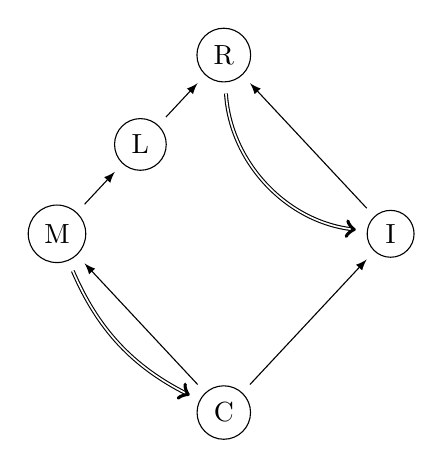
\begin{tikzpicture}[shorten <=0.4em,shorten >=0.4em]
\node [circle,draw,shift={(1ex,15ex)}] (M){M};
\node [circle,draw,shift={(15ex,0ex)}] (C){C};
\node [circle,draw,shift={(29ex,15ex)}] (I){I};
\node [circle,draw,shift={(8ex,22.5ex)}] (L){L};
\node [circle,draw,shift={(15ex,30ex)}] (R){R};
\draw [arrows={-latex}] (I) -- (R);
\draw [arrows={-latex}] (M) -- (L);
\draw [arrows={-latex}] (L) -- (R);
\draw [arrows={-latex}] (C) -- (M);
\draw [arrows={-latex}] (C) -- (I);
\draw[->,double] (M) to[bend right=20] (C);
\draw[->,double](R) to[bend right=40] (I); 
\end{tikzpicture}
\end{Scaled}
\end{minipage}
\begin{minipage}[H]{0.5\textwidth}
\begin{Scaled}{0.6}{0.6}
$
\begin{array}{|l}
\mbox{Nodes:}
\\
\begin{array}{l l}

\begin{tikzpicture}[shorten <=0.4em,shorten >=0.4em]
\node [circle,draw,shift={(0,0)}] (M){M};
\end{tikzpicture}
&\raisebox{1.5ex}{Mutable: alias, write}
\\
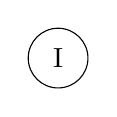
\begin{tikzpicture}[shorten <=0.4em,shorten >=0.4em]
\node [circle,draw,shift={(0,0)}] (I){${\ }$I${\ }$ };
\end{tikzpicture}
&\raisebox{1.5ex}{Immutable: alias, no write}
\\
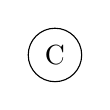
\begin{tikzpicture}[shorten <=0.4em,shorten >=0.4em]
\node [circle,draw,shift={(0,0)}] (C){C};
\end{tikzpicture}
&\parbox{50ex}{Capsule: unique access\\*
Reference used only once}
\\

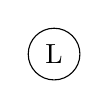
\begin{tikzpicture}[shorten <=0.4em,shorten >=0.4em]
\node [circle,draw,shift={(0,0)}] (L){L};
\end{tikzpicture}
&
\parbox{50ex}{Lent: no alias, write}
\\
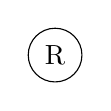
\begin{tikzpicture}[shorten <=0.4em,shorten >=0.4em]
\node [circle,draw,shift={(0,0)}] (C){R};
\end{tikzpicture}
&
\parbox{50ex}{Readable: no alias, no write}
\end{array}
\\
\mbox{Arrows:}
\\
\begin{array}{l l}
\begin{tikzpicture}
\draw [arrows={-latex}] (0,0) -- (1,0);
\end{tikzpicture}
&\mbox{Subtype}
\\
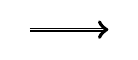
\begin{tikzpicture}
\draw[->,double] (0,0) to (1,0);
\end{tikzpicture}
&\mbox{{Recovery}}
\end{array}
\end{array}
$
\end{Scaled}
\end{minipage}
}
\caption{Type qualifiers and their relationships}
\label{fig:hierarchy}
\end{figure}
